\documentclass[12pt, a4paper]{article}
\usepackage[utf8]{inputenc}
\usepackage[english,magyar]{babel}
\usepackage[T1]{fontenc}
\usepackage[top=2.5cm, bottom=2.5cm, left=2.5cm, right=2.5cm]{geometry}

\usepackage{amsmath, mathrsfs}

\usepackage{graphicx}
\usepackage{caption}

% Define hungarian-type quote marks
\usepackage[autostyle=false]{csquotes}
\newcommand{\q}[1]{„#1''} % Redefine quotations

% Hyperlinks
\usepackage[unicode]{hyperref}
\hypersetup{
    colorlinks=true,
    linkcolor=blue,
    filecolor=magenta,
    urlcolor=cyan,
    citecolor = blue,
    pdftitle={Mikrokontroller, 2019 - Pál Balázs},
    pdfpagemode=FullScreen,
}

% Spacing and indentation
% First paragraph is indented after titles
\usepackage{indentfirst}

\setlength{\parindent}{20pt} % Indentation of paragraphs
\setlength{\parskip}{5pt}    % Skip between paragraphs (/par)

% Spacing between lines
% For 12pt normalsize, for oneandhalf we need to use
% setstretch ~ 1.241, but I'm using a rounded value of 1.25
% Other values: https://tex.stackexchange.com/questions/30073/why-is-the-linespread-factor-as-it-is
\usepackage{setspace}
%\renewcommand{\baselinestretch}{1.2}
\setstretch{1.25}

% Two columned version of text [Optional, not used!]
\usepackage{multicol}
\setlength\columnsep{30pt}

\usepackage[citestyle=authoryear, bibstyle=numeric, natbib=true, backend=bibtex, sorting=none]{biblatex}
\addbibresource{bibliography.bib}

\title{Mikrokontrollerek és alkalmazásaik laboratórium \\Év végi projektmunka -- Music box}
\author{Pál Balázs}
\date{\today}

\begin{document}

\maketitle

\section{Bevezetés}
A projekt megvalósítása során nagyvonalakban egy piezzo buzzer-t működtető kapcsolást hoztam létre, mely képes egy segédkönyvtár felhasználásával különböző zenék lejátszására. \par
Az egész projekt motivációját teljes egyszerűséggel a zenék iránti szeretetem és bármiféle hangszer birtoklásának hiánya adta. Ezeket megoldandó hoztam létre egy kapcsolást, mely képes konkrét, előre megadott hangjegyeket lejátszani és emellett egy kis \q{lézershow}-val is feldobja az egyes számokat.

\section{Megvalósítás}
A feladat elkészítéséhez egy Elegoo Uno R3 miktrokontrollert használtam, mely architektúráját tekintve megegyezik az Arduino Genuino Uno felépítésével. Az alkatrészek az ehhez tartozó \emph{The Most Complete Starter Kit} eszközgyűjtemény részét képezik. \par
A projektre készült mikrokontroller és a hozzá tartozó kapcsolási rajz sematikus ábrája a (\ref{fig:1})-es képen látható. A kapcsolásban a LED-izzókhoz $5.1 \text{k} \Omega$-os, míg a nyomógomb földeléséhez $10 \text{k} \Omega$-os ellenállásokat használtam fel. A LED-ek között szerepel egy fehér színű is, melyet csupán az állapotjelzés miatt alkalmaztam. \par
A mikrokontroller egy számítógéptől, a soros porton keresztül várja az utasításokat. A szoftver forráskódja egy \texttt{.ino} file-ból és egy hozzá tartozó \texttt{.h} könyvtárból áll. A könyvtárban a standard zenei hangmagasságoknak megfelelő elnevezések, valamint azok frekvenciái találhatóak egymáshoz rendelve. Így a forrásfile-ban elég magának a zenei hangnak a nevét megadni a \texttt{tone()} függvény számára, melyet azután az le is játszik a $11$-es portra kapcsolt piezo buzzer segítségével. \par
A forráskódba a globális változók szűkös memóriakorlátja miatt csak két zeneszámot tudtam implementálni, melyeket kották alapján dolgoztam fel. Egy harmadik zenerészlet szintén teljesen készen, azonban csak kikommentelt formában szerepel a forráskódban. Az adott zenerészlet lejátszása során a \texttt{tone()} függvény a megadott hangot egy szintén megadott időhosszik játszik le, melyet egy \texttt{delay()} függvény követ. Így biztosíthatom, hogy a kiadott zenei hang a ritmusnak megfelelően előbb véget ér és csak ezután következik a rá következő hang a lejátszásban. A \texttt{delay()} lejártával egy \texttt{notone()} függvényt is meghívok, mellyel biztosítom, hogy a hang lejátszása tényleg véget ér, és a program átfutási idejét kihasználva így biztosítom azt is, hogy az egyes hangjegyek egymástól elkülönülve hallatszódjanak az emberi fül számára. \par
A mikrokontrollerre telepített szoftver kezdetben a soros porton keresztül várja a lejátszandó zene, rövid \texttt{string} formátumú kódját. Ha a soros porton a megfelelő kód került beadásra, a miktrokotroller lejátssza a választott zeneszámot. Ezt azonban a $12$-es portra kötött nyomógomb segítségével tetszőleges időben megszakíthatjuk. Ekkor a soros porton keresztül azonnal beírhatjuk újra egy másik (vagy ugyanazon) zenerészlet kódját, lejátszva így azt.

\begin{center}
    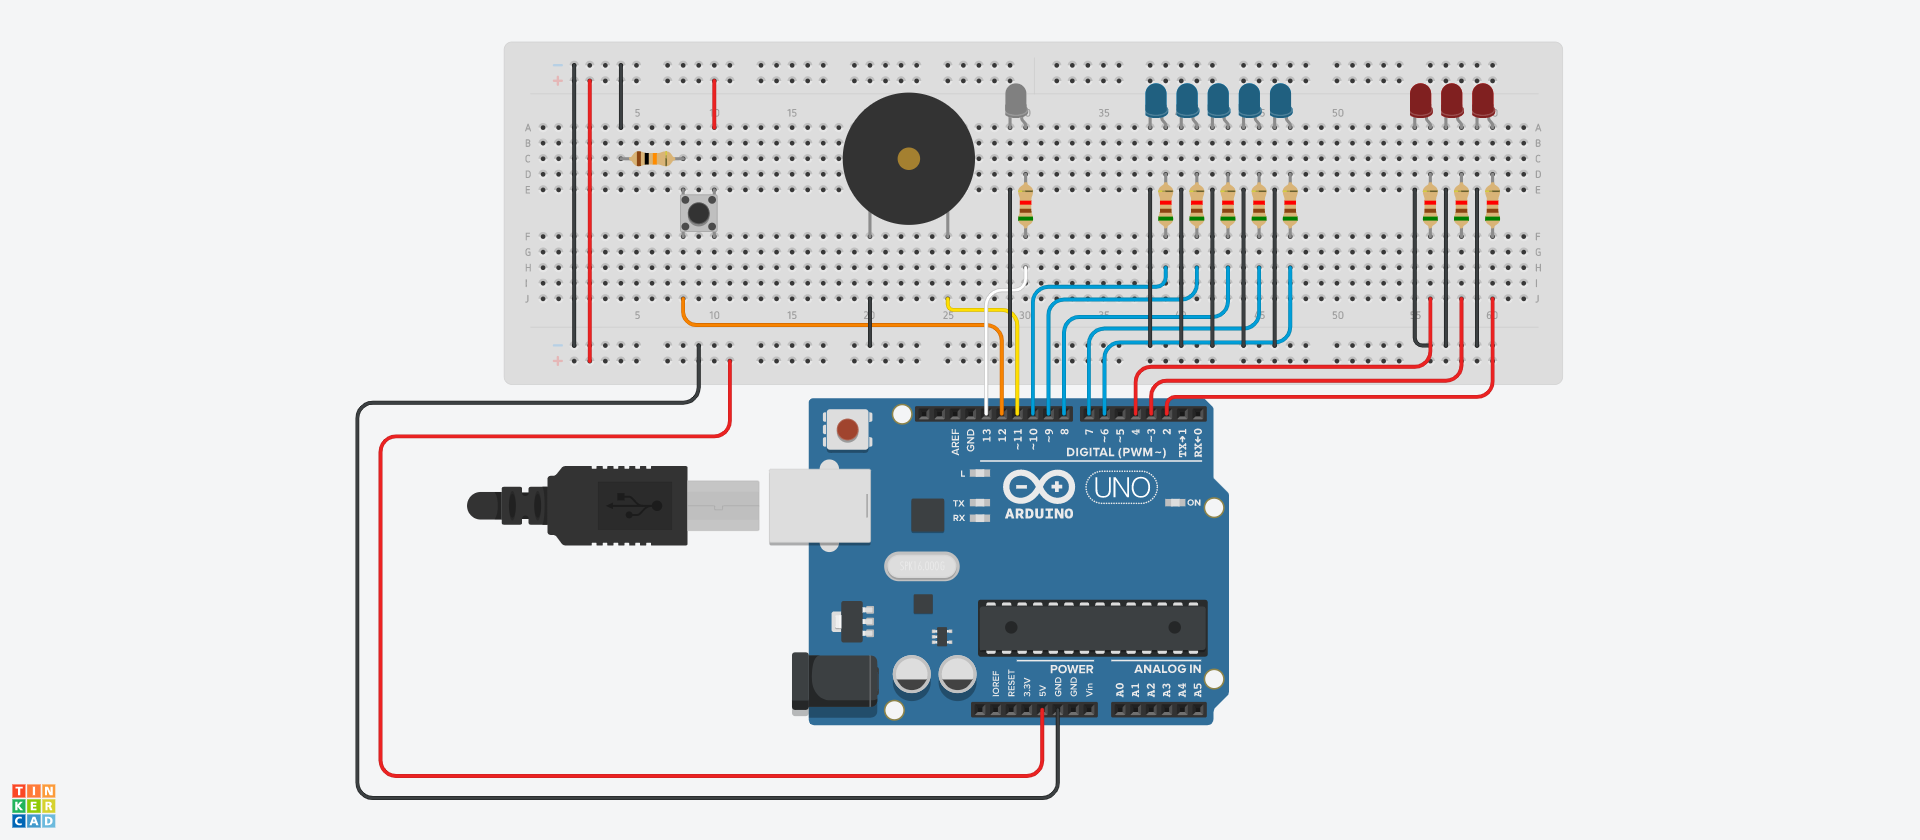
\includegraphics[width=\textwidth]{Terrific-Turing-Inari.png}
    \captionof{figure}{A mikrokontrollerhez tartozó kapcsolás szerkezete} \label{fig:1}
\end{center}
Az esztétikai hatást növelendő, az egyes számok hangulatát idéző, különböző színű és működésű LED-izzókat csatoltam a fennmaradó portokra, melyek a zene ritmusára villognak adott szabály szerint. Az egyik szám esetében a kék LED-ek közül minden hang esetében két véletlenszerű LED villan fel, így egy kaotikus fényparádét nyújtva a zene mellé. A másik szám esetében a vörös LED-eken fut végig szintén a zene ritmusára egy felvillanás sorozat. \par
A (\ref{fig:2})-es ábrán a miktrokontroller működését illusztráltam, miközben épp az egyik beprogramozott számot játssza le. A kék LED-ek közül az aktuális zenei hang lejátszása során két darab világít éppen. A távolban a fehér színű LED azt jelzi, hogy jelenleg valamelyik zene lejátszása folyik a mikrokotrolleren. Amint az adott szám véget ér, vagy a gombbal megállításra kerül, ez a LED is elalszik.

\section{Diszkusszió}
A feladat megvalósítása során végül arra koncentráltam, hogy a rendelkezésemre álló alkatrészekből egy olyan projektet alkossak, ami mind érdekel és amit élvezek is létrehozni. Ezt sikeresen teljesítettem is, melynek eredménye a jegyzőkönyvben tárgyalt eszköz és kapcsolás lett.

\begin{center}
    \includegraphics[width=\textwidth]{micro_project.png}
    \captionof{figure}{A projekt működés közben} \label{fig:2}
\end{center}

\end{document}
